\documentclass{estilo}

% --- Librerias ---
\usepackage[utf8]{inputenc}
\usepackage[spanish]{babel}
\usepackage{graphicx}
\usepackage{listings}
\usepackage{xcolor}

% --- Info ---
\title{Recuperación de información en Wikipedia}
\docauthor{Antonio Manjavacas}{Rubén Márquez}
\docdate{2019}{Octubre}

% --- Path images ---
\graphicspath{{./images/}}

\begin{document}

    \maketitle
    \tableofcontents

    \newpage
    
    \section{INTRODUCCIÓN}
    
    Los \textit{agentes de información} (también conocidos como \textit{agentes de Internet}) son un tipo de agente cuyo objetivo reside en la recolección de información a través de la red; éstos se encargan de indexarla y ofrecérsela al usuario cuando realiza una determinada consulta.
    
    Los agentes de Internet poseen un amplio rango de funcionalidades y pueden ser de lo más diversos, ya que las capacidades necesarias para la extracción de información entran dentro de las áreas de otros tipos de agentes. Surgen de la necesidad de procesar de manera automática la información y permiten facilitar el acceso a esta  aprovechando la capacidad de los agentes.

    La principal ventaja que estos agentes pueden ofrecernos, es la facilidad de acceso a información y datos no procesables manualmente.
    
    En este trabajo mostraremos un ejemplo práctico de aplicación de este tipo de agentes. El código empleado está disponible para su visualización y descarga en \url{https://github.com/manjavacas/Sistemas-Multiagente}. 
    
    \bigskip
    \section{OBJETIVOS GENERALES}
    
    El objetivo de esta práctica será la integración de servicios de tres agentes. La información obtenida por un agente web será utilizada por un agente que procese la información y una interfaz que la muestre al usuario. La estructura del sistema se detalla en la Figura \ref{fig:fig1}.

    Los agentes utilizados serán los siguientes:
    \begin{itemize}
        \item \textbf{\textit{Web agent}.} Será el agente encargado de obtener la información sobre la población histórica de Boston, Chicago y Seattle.
        \item \textbf{\textit{ProcesserAgent}.} Recibirá y procesará la información obtenida de las direcciones web. Dicho procesamiento consistirá en obtener el registro con mayor población para cada uno de los agentes y remitirlo al agente \textit{Dashboard}.
        \item \textbf{\textit{DashboardAgent}.} Se encargará de realizar peticiones de datos al \textit{ProcesserAgent} y de mostrar la información recibida al usuario.
    \end{itemize}

    \vfill
    \begin{figure} [ht]
        \centering
        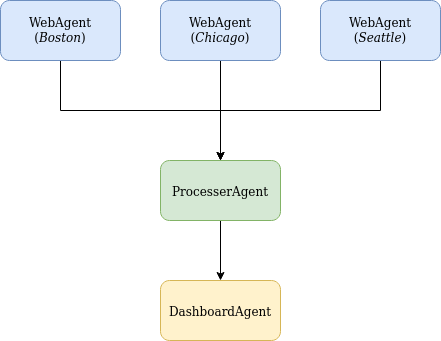
\includegraphics[width=9cm]{diagrama-agentes.png}
        \caption{Sistema multiagente a desarrollar}
        \label{fig:fig1}
    \end{figure}
    \vfill

    La información recopilada por el \textit{WebAgent} se obtendrá de las siguientes páginas de Wikipedia:

    \begin{itemize}
        \item \url{https://es.wikipedia.org/wiki/Boston}
        \item \url{https://es.wikipedia.org/wiki/Chicago}
        \item \url{https://es.wikipedia.org/wiki/Seattle}
    \end{itemize}

    \bigskip
    De dichas fuentes se recuperará la información acerca de la población histórica de las ciudades anteriormente mencionadas, la cual se encuentra en formato de tabla en el apartado \textit{Demografía} de cada una de las páginas web (un ejemplo de dichas tablas es el que se muestra en la Figura \ref{fig:fig2}). De estas tablas se obtendrán los años junto con su correspondiente población. Finalmente, el agente encargado del procesamiento de los datos obtendrá el año con mayor población histórica de cada ciudad y enviará esta información al agente \textit{Dashboard} para su presentación por pantalla.
    
    Para recuperar la información, se ha hecho uso de las librerías \textit{jsoup} (\url{https://jsoup.org/}), para obtener los ficheros HTML, y \textit{java.util.regex} para extraer la información contenida en las tablas mediante el uso de expresiones regulares. La expresión regular utilizada ha sido: \\ "\textit{\textbackslash \textbackslash d\{4\} ((\textbackslash \textbackslash s \textbackslash \textbackslash d\{4\}) | ((\textbackslash \textbackslash s \textbackslash \textbackslash d\{1,3\})\{2,3\})) \textbackslash \textbackslash s [\textbackslash \textbackslash D\&\&\textbackslash \textbackslash W]}".
    
    \begin{figure}[ht]
        \centering
        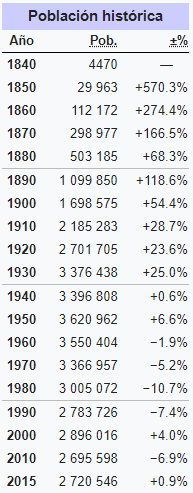
\includegraphics[scale=0.9]{table_Chicago.PNG} 
        \caption{Tabla de población histórica de Chicago}
        \label{fig:fig2}
    \end{figure}

    Por otro lado, de cara a introducir una componente aleatoria en cada uno de los agentes, se ha hecho uso de la API de \url{random.org} (\url{https://api.random.org/json-rpc/1/}) para la generación de números aleatorios. La aleatoriedad que ofrece dicha página proviene del ruido atmosférico, lo que supone que para muchos propósitos sea mejor que los algoritmos de números pseudoaleatorios ofrecidos por lenguajes de programación como Java. El funcionamiento de esta componente aleatoria consistirá en la generación de un número que decida qué registros de las tablas recuperan los agentes. 
    
    Para cada página web se generará una lista de registros del tipo [fecha, población, URL] que serán enviados al agente \textit{Processer} para que obtenga el de mayor población para cada ciudad.
    
    \bigskip
    \section{COMUNICACIÓN ENTRE AGENTES}
    
    A continuación, en la Figura \ref{fig:fig3} se detalla el flujo de comunicación entre los agentes que conforman el sistema. Nótese el uso del protocolo de comunicación FIPA-Request a la hora de realizar la solicitud de datos procesados entre \textit{Dashboard} y \textit{Processer}, así como para la obtención de los datos que ofrecen los agentes de Internet por parte del \textit{Processer}.
    
    \begin{figure}[ht]
        \centering
        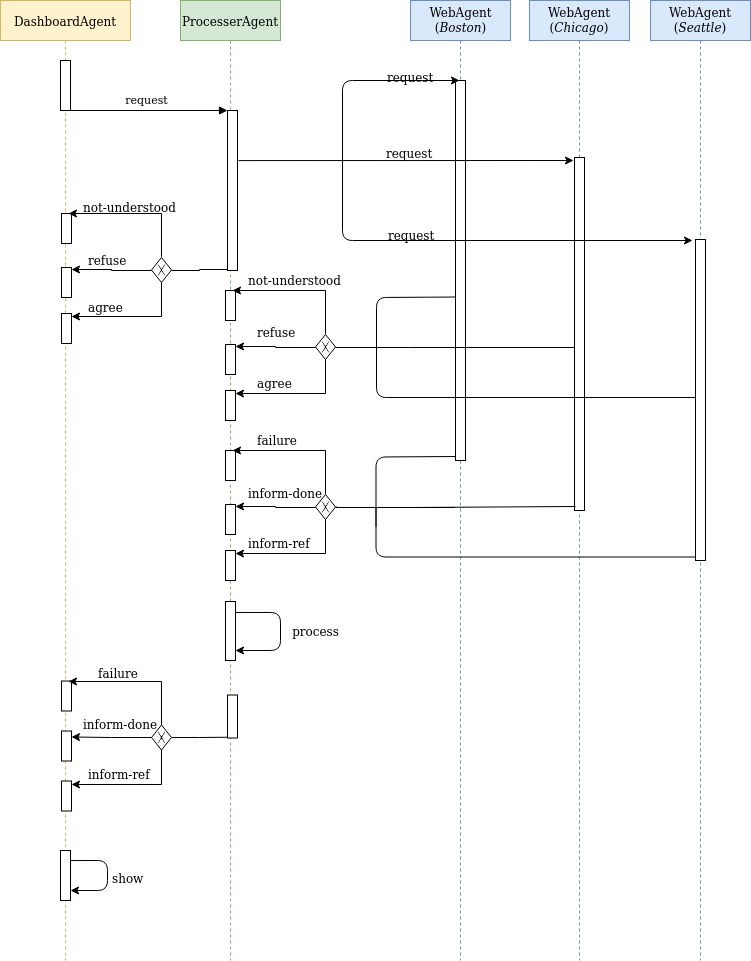
\includegraphics[scale=0.5]{images/diagrama-comunicacion.png} 
        \caption{Flujo de comunicación entre agentes}
        \label{fig:fig3}
    \end{figure}
    
    El flujo de comunicación descrito incluye:
    
    \begin{itemize}
        \item La petición del \textit{DashboardAgent} al \textit{ProcesserAgent} de los datos procesados.
        \item La petición del \textit{ProcesserAgent} al \textit{WebAgent} de la información sobre población histórica para Boston, Chicago y Seattle.
        \item La respuesta con los datos demográficos al \textit{ProcesserAgent}.
        \item La obtención del año con mayor población para cada una de las ciudades por parte del \textit{ProcesserAgent} (\textit{process}).
        \item La recepción de los datos procesados por el \textit{DashboardAgent}.
        \item La representación de dichos datos (\textit{show}).
    \end{itemize}
    
    Por otro lado, la Figura \ref{fig:fig4} incluye el diagrama de clases de diseño del sistema. Como puede observarse, cada agente incluye comportamientos y sus correspondientes manejadores para todos los tipos de mensajes definidos según el protocolo FIPA-Request:
    
    \begin{itemize}
        \item \textit{handleNotUnderstood}
        \item \textit{handleRefuse}
        \item \textit{handleAgree}
        \item \textit{handleFailure}
        \item \textit{handleInform}
        \item \textit{handleRequest}
        \item \textit{prepareResultNotification}
    \end{itemize}
    
    \begin{figure}[ht]
        \centering
        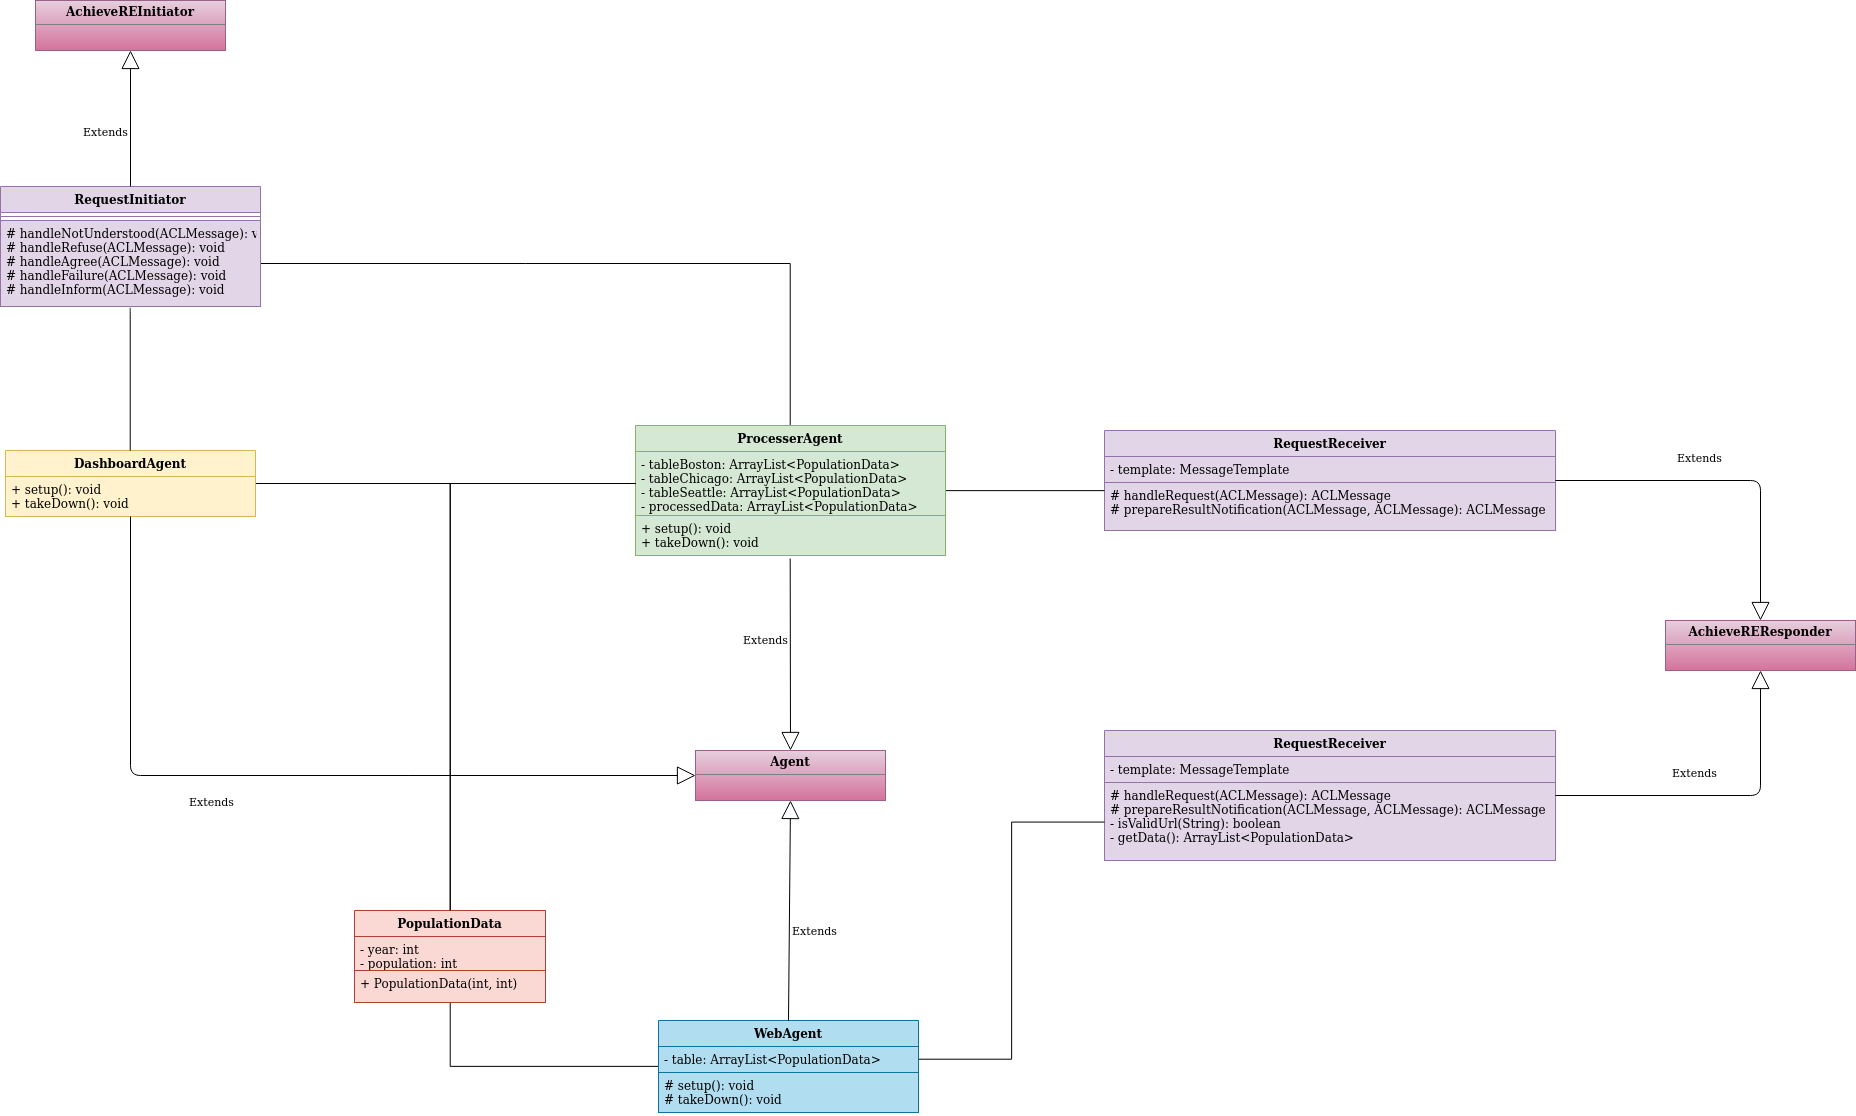
\includegraphics[scale=0.2]{images/diagrama-clases.png} 
        \caption{Diagrama de clases de diseño}
        \label{fig:fig4}
    \end{figure}
    
    \bigskip
    
    \newpage
    \section{EJECUCIÓN DEL SISTEMA}
    
    Una vez definido el comportamiento general de nuestro sistema, así como las herramientas a utilizar, veamos cómo sucede la ejecución e interacción entre agentes. El código de cada uno de ellos se encuentra incluido en la sección 5.
    
    Primero compilaremos todas las clases en el paquete \textit{agents} incluyendo las librerías en el \textit{classpath}:
    
    \begin{itemize}
        \item \textit{lib/jade.jar}
        \item \textit{lib/gson-2.8.6.jar}
        \item \textit{lib/jsoup-1.12.1.jar}
        \item \textit{lib/random-org.jar}
    \end{itemize}
    
    A continuación, iniciaremos la plataforma \textit{JADE} y crearemos cada uno de los agentes:
    
    \begin{itemize}
        \item Definiremos tres agentes del tipo \textit{WebAgent} con los nombres: \textbf{WebAgent1}, \textbf{WebAgent2} y \textbf{WebAgent3}.
        \item Nuestro \textit{ProcesserAgent} tendrá por nombre: \textbf{Processer}.
        \item Finalmente, el \textit{DashboardAgent}, con nombre: \textbf{Dashboard}.
    \end{itemize}
    
    Puede utilizarse el siguiente comando:
    \begin{lstlisting}[language=bash]
    java jade.Boot -agents WebAgent1:agents.WebAgent;
    WebAgent2:agents.WebAgent;WebAgent3:agents.WebAgent;
    Processer:agents.ProcesserAgent;Dashboard:agents.DashboardAgent
    \end{lstlisting}
    
    \subsection{\textit{DashboardAgent}}
    El comportamiento de este agente es el siguiente: al ser iniciado, despliega una interfaz gráfica con tres cuadros de texto donde el usuario puede introducir las URLs de las que se extraerá la información (ver Figura \ref{fig:fig5}). En nuestro caso, las URLs por defecto ya incluidas en la interfaz serán las correspondientes a las páginas de Wikipedia de las ciudades de Boston, Seattle y Chicago. Una vez introducidas las URLs, pulsar el botón ubicado en la esquina inferior derecha del formulario dará lugar al envío de una petición \textit{FIPA-REQUEST} al agente Processer con las URLs introducidas.
    
    Tras la obtención y procesamiento de los datos por el resto de agentes, se mostrará un segundo formulario con los datos de población histórica recibidos, reflejando los años de mayor población obtenidos para cada una de las ciudades (ver Figura \ref{fig:fig6}.
    
      \vfill
    \begin{figure} [ht]
        \centering
        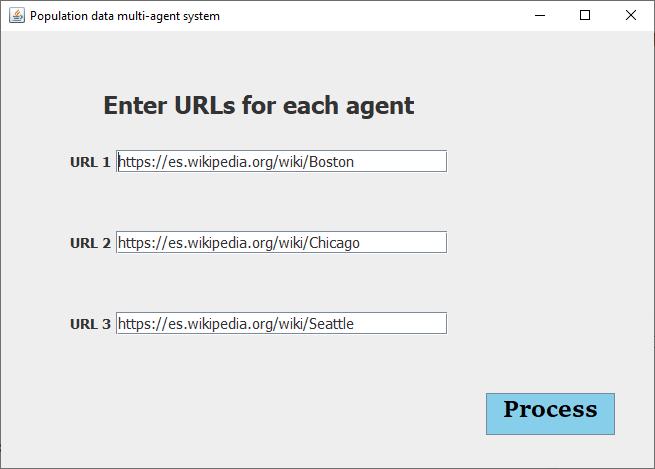
\includegraphics[width=9cm]{images/url_selection_window.PNG}
        \caption{Interfaz de usuario inicial}
        \label{fig:fig5}
    \end{figure}
    \vfill
    
    \vfill
    \begin{figure} [ht]
        \centering
        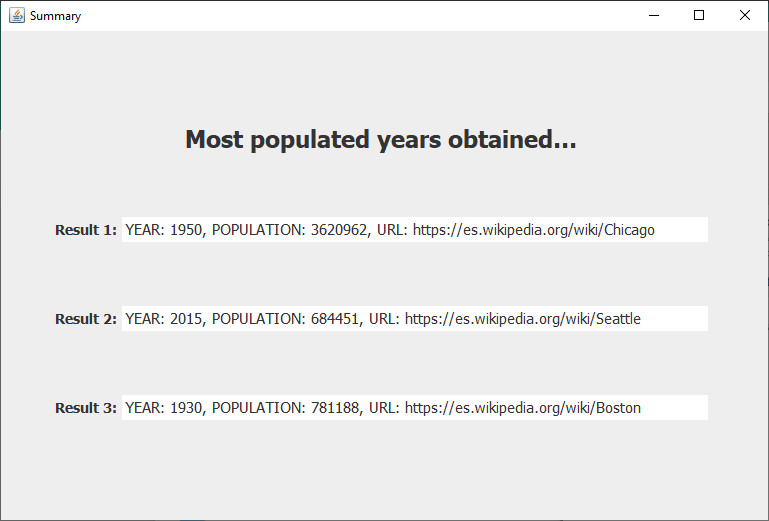
\includegraphics[width=9cm]{images/summary_window.PNG}
        \caption{Interfaz de usuario con los resultados}
        \label{fig:fig6}
    \end{figure}
    \vfill
    
    \subsection{\textit{ProcesserAgent}}
    Este agente actuará como intermediario entre la interfaz y el agente de Internet. Cuando el Processer recibe una petición \textit{FIPA-REQUEST} del Dashboard, obtiene las tres URLs contenidas en el mensaje y genera las peticiones de tipo \textit{FIPA-REQUEST} que envía a cada uno de los agentes de Internet por medio de un comportamiento compuesto. Dicho comportamiento, ya sea paralelo o secuencial, estará compuesto por tres subcomportamientos del tipo AchieveREInitiator, que enviarán una URL a cada \textit{WebAgent}. 
    
    La comparación en el orden de envío y recepción de mensajes según el tipo de comportamiento compuesto empleado puede observarse en las figuras Figura \ref{fig:fig7} y Figura \ref{fig:fig8}.
    
    Una problemática ante la que nos encontramos fue la necesidad de esperar a la respuesta de todos los agentes web antes de responder al Dashboard. Como puede observarse en el código, fue necesario redefinir el método \textit{prepareResultNotification(ACLMessage request, ACLMessage response)} del AchieveREResponder mediante \textit{registerPrepareResultNotification(Behaviour b)} y acceder directamente al DataStore (cola de mensajes) del comportamiento AchieveREResponder para introducir la respuesta al Dashboard solamente cuando los agentes web hubiesen terminado su tarea.
    
    \vfill
    \begin{figure} [ht]
        \centering
        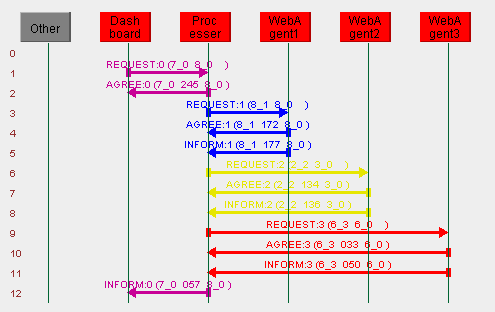
\includegraphics[width=9cm]{images/sniffer_capture_sequential.PNG}
        \caption{Intercambio de mensajes con comportamiento secuencial}
        \label{fig:fig7}
    \end{figure}
    \vfill
    
    \vfill
    \begin{figure} [ht]
        \centering
        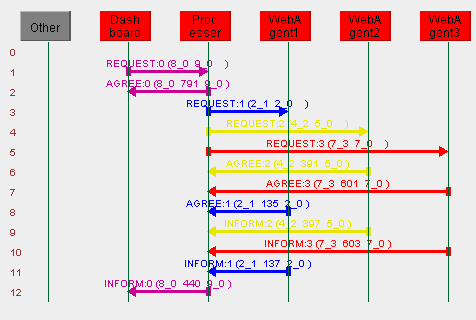
\includegraphics[width=9cm]{images/sniffer_capture_parallel.PNG}
        \caption{Intercambio de mensajes con comportamiento paralelo}
        \label{fig:fig8}
    \end{figure}
    \vfill
    
   Una vez recibidas todas las respuestas de los agentes web, el Processer obtiene los registros con mayor población para cada URL y responde al Dashboard con los datos obtenidos.
    
    \subsection{\textit{WebAgent}}
    Las peticiones del Processer son recibidas por los agentes web: WebAgent1, WebAgent2 y WebAgent3. Dichos agentes extraen los datos asociados a la URL recibida mediante el método \textit{getData()}, que almacena cada uno de los registros de las tablas de población histórica en objetos del tipo PopulationData. Finalmente, el conjunto de registros se envía en un mensaje de respuesta al Processer.
    
    \newpage
    \section{CLASES EMPLEADAS}
    
    \definecolor{codegreen}{rgb}{0,0.6,0}
    \definecolor{codegray}{rgb}{0.5,0.5,0.5}
    \definecolor{codepurple}{rgb}{0.58,0,0.82}
    \definecolor{backcolour}{rgb}{0.95,0.95,0.92}
    
    \lstdefinestyle{mystyle}{
        backgroundcolor=\color{backcolour},   
        commentstyle=\color{codegreen},
        keywordstyle=\color{magenta},
        numberstyle=\tiny\color{codegray},
        stringstyle=\color{codepurple},
        basicstyle=\footnotesize,
        breakatwhitespace=false,         
        breaklines=true,                 
        captionpos=b,                    
        keepspaces=true,                 
        numbers=left,                    
        numbersep=5pt,                  
        showspaces=false,                
        showstringspaces=false,
        showtabs=false,                  
        tabsize=2
    }
 
    \lstset{style=mystyle}
    
    \vspace{0.5cm}
    \centering{Clase \textit{DashboardAgent}: implementa la interfaz con el usuario y la petición de los datos}
    \lstinputlisting[language=Java]{./code/DashboardAgent.java}
    
    \newpage
    \centering{Clase \textit{ProcesserAgent}: intermediario entre agentes encargado de procesar los datos de la web}
    \lstinputlisting[language=Java]{./code/ProcesserAgent.java}
    
    \newpage
    \centering{Clase \textit{WebAgent}: agente de Internet}
    \lstinputlisting[language=Java]{./code/WebAgent.java}
    
    \newpage
    \centering{Clase \textit{PopulationData}: representa los registros de población anual obtenidos}
    \lstinputlisting[language=Java]{./code/PopulationData.java}

\end{document}
    